\documentclass[12pt]{article}
\usepackage{graphicx}
\usepackage{amsmath,amssymb}
\usepackage{hyperref}
\usepackage{fontspec}
\usepackage{setspace}
\usepackage[margin=1in]{geometry}
\usepackage[table,xcdraw]{xcolor}
\usepackage[textfont={rm,it}]{caption}
\usepackage{subcaption}
\usepackage{subfloat}
\usepackage{multirow}
\usepackage{multicol}
\usepackage[american]{babel}
\usepackage{csquotes}

\begin{document}
\title{Yizhong Hu Summer 2023 Results Report}
\author{Yizhong Hu}
\maketitle

\section{Jun 1 - Jun 5}

\subsection{Model Description}

We consider the Hamiltonian $\mathcal{H}: \mathcal{X}^{\kappa + 1} \times \mathcal{Y}^{\kappa} \mapsto \mathbb{R}$

\begin{equation*}
    \mathcal{H}(x_0, x_1, \ldots, x_\kappa, y_{01}, \ldots, y_{0\kappa} ) = \frac{\beta}{2}\sum_{i=1}^\kappa x_0x_iy_{0i} + Bx_0
\end{equation*}
where $x_0$ is spin state of the root node, $x_i$ is the spin state of the $i$-th leaf node, $y_{0i}$ is the interaction between
$0$ and $i$. All of them take values in $\mathcal{X} = \mathcal{Y} = \{-1, 1\}$.

When $\kappa=2$,
\begin{equation*}
    \mathcal{H}(x_0, x_1, x_2, y_{01}, y_{02} ) = \frac{\beta}{2}(x_0x_1y_{01} + x_0x_2y_{02}) + Bx_0
\end{equation*}

We define the state $s$ in state space $\mathbb{S} = \mathcal{X}^3 \times \mathcal{Y}^2$, and the random variable $S$ a random variable
on $\mathbb{S}$. Given $\eta$ the i.i.d Bernoulli(1/2) distribution on $\mathbb{S}$, we want to investigate the distribution $\mu(\cdot)$ that maximizes
\begin{equation*}
    \max_{\mu(\cdot)} \left\{\mathbb{E}_\mu[\mathcal{H}(S)] - \left[H(\mu \| \eta) + H(\mu_{01}\|\eta_{01} )\right]\right\}
\end{equation*}

\subsection{Analytical analysis}

First, we need to find the distribution $\mu: \mathcal{X}^3 \times \mathcal{Y}^2 \mapsto [0, 1]$. Since the input is discrete,
$\mu$ can be rewritten as a vector on $[0, 1]^{2^5}$. We will denote each component as $\mu(s)$, with $s\in \mathbb{S}$

The marginal distribution is therefore
\begin{equation*}
    \mu_{01}(y_{01}) = \sum_{x_1, x_2, x_3, y_{02} \in \{-1, 1\}} \mu(s)
\end{equation*}

Rewriting each term,
\begin{align*}
    \mathbb{E}_\mu[\mathcal{H}(S)] & = \sum_{s\in \mathbb{S}} \mu(s) \mathcal{H}(s)                                                 \\
    H(\mu \| \eta)                 & = \sum_{s\in \mathbb{S}} \mu(s) \log\frac{\mu(s)}{\eta(s)}                                     \\
    H(\mu_{01} \| \eta_{01})       & = \sum_{y_{01}\in \mathcal{Y}} \mu_{01}(y_{01}) \log\frac{\mu_{01}(y_{01})}{\eta_{01}(y_{01})}
\end{align*}
Note that since $\eta$ is uniform, the relative entropies can be written directly in terms of their entropies:
\begin{align*}
    H(\mu \| \eta)           & = H(\mu) - \log |\mathbb{S}| \\
    H(\mu_{01} \| \eta_{01}) & = H(\mu_{01}) - \log 2
\end{align*}
Rewriting the target,
\begin{equation*}
    \max_{\mu(\cdot)} \left[\sum_{s\in \mathbb{S}} \mu(s) \mathcal{H}(s) - \sum_{s\in \mathbb{S}} \mu(s) \log \mu(s) + \sum_{y_{01}\in \mathcal{Y}} \mu_{01}(y_{01}) \log\mu_{01}(y_{01})\right]
\end{equation*}

The corresponding Lagrange multiplier (constrained on $\mu$ being normalized) is
\begin{equation*}
    \mathcal{L} =\left[\sum_{s\in \mathbb{S}} \mu(s) \mathcal{H}(s) - \sum_{s\in \mathbb{S}} \mu(s) \log \mu(s) + \sum_{y_{01}\in \mathcal{Y}} \mu_{01}(y_{01}) \log\mu_{01}(y_{01})\right] + \lambda\left[\sum_{s\in \mathbb{S}} \mu(s) - 1\right]
\end{equation*}
taking the gradients gives
\begin{align}
    \frac{\partial \mathcal{L}}{\partial \mu(s)}  & = \mathcal{H}(s) - \log \mu(s) + \log \mu_{01}(y_{01}) + \lambda = 0 \\
    \frac{\partial \mathcal{L}}{\partial \lambda} & = \sum_{s\in \mathbb{S}} \mu(s) - 1 = 0
\end{align}
where $y_{01}$ in Eq.(1) represents the value of $y_{01}$ in $s$.

Eq.(1) gives the form of $\mu$ in terms of a conditional distribution, as seen below:
\begin{align*}
    \log \mu(s) - \log \mu_{01}(y_{01})  & = \mathcal{H}(s) + \lambda     \\
    \log \frac{\mu(s)}{\mu_{01}(y_{01})} & = \mathcal{H}(s) + \lambda     \\
    \frac{\mu(s)}{\mu_{01}(y_{01})}      & = e^\lambda e^{\mathcal{H}(s)}
\end{align*}
The left-hand side is a conditional distribution:
\begin{equation}
    \mathbb{P}_\mu (S = s | Y_{01} = y_{01}) = \frac1Z \exp\left[\frac{\beta}{2}(x_0x_1y_{01} + x_0x_2y_{02}) + Bx_0\right]
\end{equation}
for some $Z = e^{-\lambda} = $ normalizing constant.

Since $\frac{\partial \mathcal{L}}{\partial \mu(s)} = 0$ for all $\mu_{01}$ values, and all such optimum points form a connected curve,
we think that it is reasonable to hypothesize that any choice of $\mu_{01}$ satisfies optimality.
Since $y_{01}$ can only take two values, the distribution can be characterized by a single real value $\alpha$:
\begin{equation*}
    \mathbb{P}_\mu(Y_{01} = y_{01}) = \frac{e^{\alpha y_{01}}}{e^\alpha + e^{-\alpha}},
\end{equation*}
and the entire distribution becomes
\begin{equation*}
    \mu(s) = \frac1Z \exp\left[\frac{\beta}{2}(x_0x_1y_{01} + x_0x_2y_{02}) + Bx_0 + \alpha y_{01}\right]
\end{equation*}

\subsection{Numerical Analysis}

On the other hand, this problem can be solved numerically, formulated as a constrained optimization:

\begin{align*}
    \text{maximize}\quad   & \sum_{s\in \mathbb{S}} \mu(s) \mathcal{H}(s) - \sum_{s\in \mathbb{S}} \mu(s) \log \mu(s) + \sum_{y_{01}\in \mathcal{Y}} \mu_{01}(y_{01}) \log\mu_{01}(y_{01}) \\
    \text{subject to}\quad & \sum_{s\in\mathbb{S}} \mu(s) = 1
\end{align*}

Since entropy calculations really don't like getting negative values, we will represent $\mu$ as an exponential:
\begin{equation*}
    \mu(s) = e^{x(s)}
\end{equation*}
Note that since $\exp: \mathbb{R} \mapsto (0, \infty)$ is bijective, we do not lose any generality.

A proximal point optimization method will be used for the optimization. For the following optimization problem

$$\begin{aligned}
        \text{maximize}\quad   & f(\textbf{x})                        \\
        \text{subject to}\quad & \textbf{g}(\textbf{x}) = \textbf{0},
    \end{aligned}$$
we have the following iterative process to obtain an optimum:
$$\begin{aligned}
        \textbf{x}^{(t+1)}       & = \text{argmax}_{\text{x}} f(\text{x}) + \mathbf{\lambda}^{(t)} \cdot \textbf{g}(\textbf{x}) - \frac12 (\textbf{g}(\textbf{x}))^2 \\
        \mathbf{\lambda}^{(t+1)} & = \mathbf{\lambda}^{(t)} - \textbf{g}\left(\textbf{x}^{(t+1)}\right)                                                              \\
    \end{aligned}$$
The minimization on $\textbf{x}$ is done with the SciPy minimize. The code is provided in the notebook attached.

Results from numerical analysis confirm the results from analytical analysis. Aside from inaccuracies introduced by low value of $\mu_{01}(y_{01})$,
the conditional distribution given $Y_{01}$ matches the exponential distribution $\exp[\mathcal{H}(s)]$ to around $10^{-6}$ accuracy. Additionally,
any distribution on $Y_{01}$ can be optimal, which conforms with the analytical understanding.

\subsection{Correlation}

To see the correlation, we will try to calculate the Pearson coefficient for the pairs of random variables. We will test these on different choices of $\beta$ and $B$. To make sure that the results are accurate, we reduced the accuracy requirement to below $10^{-10}$.

\begin{itemize}
    \item For $Y^*_{01}$, and $X^*_{0}$, we can see that the Pearson coefficient is very close to $0$ except for when $B$ is much larger than $1$ and $Y^*_{01}$
          is skewed to one of the results, which could be just an accuracy issue. We hence hypothesize that $Y^*_{01}$, and $X^*_{0}$ are independent.
          To make it more certain, we can try numerically calculating the distribution in exponential form to confirm.
\end{itemize}




It is unclear what correlation is like in this situation. Given how the distribution is structured, we can separate the exponent additively to obtain
mutually independent pieces. For example, if we fix $x_0$, we know that $X_1, Y_{01}$ and $X_2, Y_{02}$ are independent of each other:
\begin{equation*}
    \mu(s) = \frac1Z \exp(Bx_0) \exp\left[\frac{\beta}{2}(x_0x_1y_{01}) + \alpha y_{01}\right] \exp\left[ \frac\beta2 x_0x_2y_{02}\right]
\end{equation*}
I have tried to calculate the covariance between different random variables from the numerical results, but they differ by the choice of $\mu_{01}$,
and the marginal distributions don't seem like there is a definitive answer for if they correlate or are independent. I may need more guidance on this
issue.

\newpage

\section{Jun 6 - Jun 12}

To simplify, we still consider the Ising model.

\subsection{Numerical Analysis}

\subsubsection{Method}

We vectorize the state, representing the probability as $\mu_{x_0k}$, where $x_0$ is the spin state for the root node, and $k$ leaves
are in the spin-up state. The Hamiltonian can then be rewritten
\begin{equation*}
    \mathcal{H}(x_0, k) = \frac{\beta}{2}x_0(2k-\kappa) + Bx_0.
\end{equation*}
The edge distribution is therefore, for some distribution $p$,
\begin{equation*}
    \pi_p(x_0, x_v)=\frac1\kappa\sum_{k=1}^\kappa p_{x_0k}\left[\mathbf{1}_{\{x_v=1\}}k + \mathbf{1}_{\{x_v=-1\}}(\kappa-k)\right].
\end{equation*}
Note that if we represent $\mu\in\mathbb{R}^{2\times {(\kappa+1)}}$, this can be represented as a matrix multiplication.

The underlying distribution needs to account for multiplicity as well:
\begin{equation*}
    \eta_{x_0k} = {\kappa \choose k} 2^{-\kappa}.
\end{equation*}
Hence, the optimization problem becomes
\begin{align*}
    \text{maximize}\quad   & \sum_{x_0\in\mathcal{X}}\sum_{k=0}^\kappa \mu_{x_0k}\mathcal{H}(x_0, k) - \sum_{x_0\in\mathcal{X}}\sum_{k=0}^\kappa \mu_{x_0k}\log\frac{\mu_{x_0k}}{\eta_{x_0k}} + \frac{\kappa}{2} \sum_{x_0\in\mathcal{X}}\sum_{x_v\in\mathcal{X}} \pi_\mu(x_0, x_v)\log\frac{\pi_\mu(x_0, x_v)}{\pi_\eta(x_0, x_v)} \\
    \text{subject to}\quad & \sum_{x_0\in\mathcal{X}}\sum_{k=0}^\kappa \mu_{x_0k} = 1                                                                                                                                                                                                                                               \\
                           & \pi_\mu(1, -1) = \pi_\mu(-1, 1).
\end{align*}
Like last time, to guarantee positivity, we instead optimize for some $\xi$ such that $\mu_{x_0k} = \exp(\xi_{x_0k})$. And again,
we optimize with a proximal point method. Proximal points are calculated with L-BFGS-B from SciPy. The tolerances of the optimization target, $\mu^*$, and constraints are $10^{-6}$.

\pagebreak

\subsubsection{Objects of interest}

\begin{itemize}
    \item First consider $X_0$ and $X_1$, where $X_1$ is a leaf chosen uniformly. The joint distribution is
          \begin{equation*}
              \mathbb{P}_{\mu}(X_0=x_0, X_1=x_1) = \pi_\mu(x_0, x_1).
          \end{equation*}
          Since $\pi_\mu(x_0, x_1)$ is symmetric, they are identically distributed.
          From numerical analysis, we find that only when $\beta$ is $0$ are $X_0$ and $X_1$ independent.
          When $\beta > 0$, there is a preference of $X_0$ and $X_1$ being the same spins, and vice versa.
          For $B=0$, As $|\beta| \rightarrow \infty$, we see that $X_0$ and $X_1$ goes to Bernoulli(1/2).
    \item Then we consider $X_1$ and $X_2$, where they are distinct leaves chosen uniformly:
          \begin{equation*}
              \mathbb{P}_{\mu}(X_1=x_1, X_2=x_2) = \frac{1}{{\kappa \choose k}} \sum_{x_0\in\mathcal{X}} \mu_{x_0k} ,
          \end{equation*}
          where $k$ is the number of spin-up states in $\{x_1, x_2\}$
          % \begin{equation*}
          %     \nu(x_1, x_2; \kappa, k) = \mathbb{P}_{\mu}(X_1=x_1, X_2=x_2 | k) = \frac{1}{{\kappa \choose 2}}\begin{cases}
          %         {k \choose 2} & x_1=x_2=1 \\
          %         \frac12{k \choose 1}{\kappa - k \choose 1} & x_1\neq x_2 \\
          %         {\kappa - k \choose 2} & x_1=x_2=-1 
          %     \end{cases}
          % \end{equation*}
          Results from the simulation conclude that $X_1$ and $X_2$ are only independent when $\beta=0$. The higher the $\beta$
          is, we approach $X_1=X_2$.
    \item For $X_1$ and $X_2$ conditioned under $X_0$, we have
          \begin{equation*}
              \mathbb{P}_{\mu}(X_1=x_1, X_2=x_2 | X_0 = x_0) = \frac{1}{{\kappa \choose k}} \mu_{x_0k}.
          \end{equation*}
          Again, $X_1$ and $X_2$ are only independent when $\beta=0$. When $\beta>0$, they tend to equal $X_0$, and when $\beta<0$,
          they tend to equal $-X_0$, consistent with the first conclusion.
\end{itemize}

This points towards a representation of $\mu^*$ similar to the form
\begin{equation*}
    \mu^*(x_0, x_1, x_2) = \frac1Z\exp(\mathcal{H}(x_0, x_1, x_2)).
\end{equation*}


\subsection{Analytical solution}

The corresponding Lagrange multiplier is
\begin{multline*}
    \mathcal{L} = \sum_{x_0\in\mathcal{X}}\sum_{k=0}^\kappa \mu_{x_0k}\mathcal{H}(x_0, k)
    - \sum_{x_0\in\mathcal{X}}\sum_{k=0}^\kappa \mu_{x_0k}\log\frac{\mu_{x_0k}}{\eta_{x_0k}}
    + \frac{\kappa}{2} \sum_{x_0\in\mathcal{X}}\sum_{x_v\in\mathcal{X}} \pi_\mu(x_0, x_v)\log\frac{\pi_\mu(x_0, x_v)}{\pi_\eta(x_0, x_v)} \\
    + \lambda_1 \left(\sum_{x_0\in\mathcal{X}}\sum_{k=0}^\kappa \mu_{x_0k} - 1\right)
    + \lambda_2 \left[\pi_\mu(-1, 1) - \pi_\mu(1, -1)\right].
\end{multline*}
To take partial derivatives, first note that
\begin{align*}
    \frac{\partial \pi_\mu(x_0, 1)}{\partial \mu_{x_0k}}  & = \frac{k}{\kappa}           \\
    \frac{\partial \pi_\mu(x_0, -1)}{\partial \mu_{x_0k}} & = \frac{\kappa - k}{\kappa}.
\end{align*}
Then, we have
\begin{multline*}
    \frac{\partial \mathcal{L}}{\partial \mu_{x_0k}} = \mathcal{H}(x_0, k)
    - \log\frac{\mu_{x_0k}}{\eta_{x_0k}} - 1
    + \frac{\kappa}{2}\left\{
    \left[\log\frac{\pi_\mu(x_0, 1)}{\pi_\eta(x_0, 1)}+1\right]\frac{k}{\kappa} +
    \left[\log\frac{\pi_\mu(x_0, -1)}{\pi_\eta(x_0, 1)}+1\right]\frac{\kappa - k}{\kappa}
    \right\} \\
    + \lambda_1
    + \lambda_2 \left(\mathbf{1}_{\{x_0=1\}}\frac{\kappa - k}{\kappa} -
    \mathbf{1}_{\{x_0=-1\}}\frac{k}{\kappa}\right) = 0,
\end{multline*}
which can be simplified to
\begin{multline*}
    \log\frac{\mu_{x_0k}}{\eta_{x_0k}} = \mathcal{H}(x_0, k)
    + \frac{1}{2}\left[
        k\log\frac{\pi_\mu(x_0, 1)}{\pi_\eta(x_0, 1)} +
        (\kappa - k)\log\frac{\pi_\mu(x_0, -1)}{\pi_\eta(x_0, 1)}
        \right] + \frac{\kappa}{2} - 1\\
    + \lambda_1
    + \lambda_2 \left(\mathbf{1}_{\{x_0=1\}}\frac{\kappa - k}{\kappa} -
    \mathbf{1}_{\{x_0=-1\}}\frac{k}{\kappa}\right)
\end{multline*}
Hence, we can conclude
\begin{equation*}
    \mu_{x_0k} = \frac1Z \eta_{x_0k} \left[\frac{\pi_\mu(x_0, 1)}{\pi_\eta(x_0, 1)}\right]^{k/2} \left[\frac{\pi_\mu(x_0, -1)}{\pi_\eta(x_0, 1)}\right]^{(\kappa - k)/2} \exp\left[\mathcal{H}(x_0, k) + \lambda_2 \left(\mathbf{1}_{\{x_0=1\}}\frac{\kappa - k}{\kappa} -
        \mathbf{1}_{\{x_0=-1\}}\frac{k}{\kappa}\right)\right]
\end{equation*}
where
\begin{equation*}
    Z = \sum_{x_0\in\mathcal{X}}\sum_{k=0}^\kappa \eta_{x_0k} \eta_{x_0k} \left[\frac{\pi_\mu(x_0, 1)}{\pi_\eta(x_0, 1)}\right]^{k/2} \left[\frac{\pi_\mu(x_0, -1)}{\pi_\eta(x_0, 1)}\right]^{(\kappa - k)/2} \exp\left[\mathcal{H}(x_0, k) + \lambda_2 \left(\mathbf{1}_{\{x_0=1\}}\frac{\kappa - k}{\kappa} -
        \mathbf{1}_{\{x_0=-1\}}\frac{k}{\kappa}\right)\right]
\end{equation*}
This is, however, not a closed-form solution, as $\pi_\mu$ is still a linear combination of elements in $\mu$

\pagebreak

\section{Jun 14 - Jun 20}

\subsection{Objects of interest}

A proximal point method was used, but it may not be as reliable as some SciPy implementations. SLSQP is used instead
to find the optimum. This guarantees that all the guesses satisfy constraints. The tolerance for the objective function is $10^{-10}$.
This seems to result in $\mu^*$ that is accurate to $10^{-5}$.

\subsubsection{Investigating $\mathbb{P}_{\mu^*}(X_0, X_v)$}

As mentioned, we know that $\mathbb{P}_{\mu^*}(X_0=x_0, X_v=x_v) = \pi_{\mu^*}(x_0, x_v)$
For independence, we need to show that
\begin{equation*}
    \mathbb{P}_{\mu^*}(X_0=x_0, X_v=x_v) =  \mathbb{P}_{\mu^*}(X_0=x_0) \mathbb{P}_{\mu^*}(X_v=x_v)
\end{equation*}

When $\beta=0$, $X_0$ and $X_v$ are independent (Tab.\ref{Tab. beta0B0}):
\begin{table}[h]
    \centering
    \begin{tabular}{c|rr}
        $\mathbb{P}_{\mu^*}(X_0, X_v)$ & \multicolumn{1}{c}{$X_v=-1$} & \multicolumn{1}{c}{$X_v=1$} \\ \hline
        $X_0=-1$                       & 0.25                         & 0.25                        \\
        $X_0=1$                        & 0.25                         & 0.25
    \end{tabular}
    \quad\quad
    \begin{tabular}{c|rr}
        $\mathbb{P}_{\mu^*}(X_0)\mathbb{P}_{\mu^*}(X_v)$ & \multicolumn{1}{c}{$X_v=-1$} & \multicolumn{1}{c}{$X_v=1$} \\ \hline
        $X_0=-1$                                         & 0.25                         & 0.25                        \\
        $X_0=1$                                          & 0.25                         & 0.25
    \end{tabular}
    \caption{When $\beta=0$ and $B=0$, up to $10^{-5}$ accuracy, the product of the marginals is equal to the join distribution}
    \label{Tab. beta0B0}
\end{table}

\noindent The higher the value for $\beta$, the more correlated $X_0$ and $X_v$ are. As $\beta\rightarrow\infty$, the correlation becomes stronger,
approaching $X_0=X_v$ (Tab.\ref{Tab. beta-higher-B0}).

\begin{table}[h]
    \raggedright
    $\beta=1$\\
    \centering
    \begin{tabular}{c|rr}
        $\mathbb{P}_{\mu^*}(X_0, X_v)$ & \multicolumn{1}{c}{$X_v=-1$} & \multicolumn{1}{c}{$X_v=1$} \\ \hline
        $X_0=-1$                       & 0.44                         & 0.06                        \\
        $X_0=1$                        & 0.06                         & 0.44
    \end{tabular}
    \quad\quad
    \begin{tabular}{c|rr}
        $\mathbb{P}_{\mu^*}(X_0)\mathbb{P}_{\mu^*}(X_v)$ & \multicolumn{1}{c}{$X_v=-1$} & \multicolumn{1}{c}{$X_v=1$} \\ \hline
        $X_0=-1$                                         & 0.25                         & 0.25                        \\
        $X_0=1$                                          & 0.25                         & 0.25
    \end{tabular} \\
    \raggedright
    $\beta=3$\\
    \centering
    \begin{tabular}{c|rr}
        $\mathbb{P}_{\mu^*}(X_0, X_v)$ & \multicolumn{1}{c}{$X_v=-1$} & \multicolumn{1}{c}{$X_v=1$} \\ \hline
        $X_0=-1$                       & 0.499                        & 0.001                       \\
        $X_0=1$                        & 0.001                        & 0.499
    \end{tabular}
    \quad\quad
    \begin{tabular}{c|rr}
        $\mathbb{P}_{\mu^*}(X_0)\mathbb{P}_{\mu^*}(X_v)$ & \multicolumn{1}{c}{$X_v=-1$} & \multicolumn{1}{c}{$X_v=1$} \\ \hline
        $X_0=-1$                                         & 0.25                         & 0.25                        \\
        $X_0=1$                                          & 0.25                         & 0.25
    \end{tabular} \\
    \raggedright
    $\beta=10$\\
    \centering
    \begin{tabular}{c|rr}
        $\mathbb{P}_{\mu^*}(X_0, X_v)$ & \multicolumn{1}{c}{$X_v=-1$} & \multicolumn{1}{c}{$X_v=1$} \\ \hline
        $X_0=-1$                       & 0.50                         & 0.00                        \\
        $X_0=1$                        & 0.00                         & 0.50
    \end{tabular}
    \quad\quad
    \begin{tabular}{c|rr}
        $\mathbb{P}_{\mu^*}(X_0)\mathbb{P}_{\mu^*}(X_v)$ & \multicolumn{1}{c}{$X_v=-1$} & \multicolumn{1}{c}{$X_v=1$} \\ \hline
        $X_0=-1$                                         & 0.25                         & 0.25                        \\
        $X_0=1$                                          & 0.25                         & 0.25
    \end{tabular}
    \caption{$\beta$ takes values 1, 3, and 10 and $B=0$. Notice that
        as $\beta$ increases, the correlation between $X_0$ and $X_v$ becomes stronger. They are no longer independent. They are positively correlated, i.e. $0$ and $v$ prefer being in the same
        state. It is hence reasonable to postulate that as $\beta\rightarrow\infty$, we will have $X_0=X_v$}
    \label{Tab. beta-higher-B0}
\end{table}

\noindent If $\beta < 0$, $X_0$ and $X_v$ are negatively correlated, and again, as $|\beta|\rightarrow \infty$, the correlation becomes stronger,
approaching $X_0=-X_v$ (Tab.\ref{Tab. beta-neg-B0}).

\begin{table}[h]
    \raggedright
    $\beta=-1$\\
    \centering
    \begin{tabular}{c|rr}
        $\mathbb{P}_{\mu^*}(X_0, X_v)$ & \multicolumn{1}{c}{$X_v=-1$} & \multicolumn{1}{c}{$X_v=1$} \\ \hline
        $X_0=-1$                       & 0.060                        & 0.440                       \\
        $X_0=1$                        & 0.440                        & 0.0596
    \end{tabular}
    \quad\quad
    \begin{tabular}{c|rr}
        $\mathbb{P}_{\mu^*}(X_0)\mathbb{P}_{\mu^*}(X_v)$ & \multicolumn{1}{c}{$X_v=-1$} & \multicolumn{1}{c}{$X_v=1$} \\ \hline
        $X_0=-1$                                         & 0.250                        & 0.250                       \\
        $X_0=1$                                          & 0.250                        & 0.250
    \end{tabular} \\
    \raggedright
    $\beta=-3$\\
    \centering
    \begin{tabular}{c|rr}
        $\mathbb{P}_{\mu^*}(X_0, X_v)$ & \multicolumn{1}{c}{$X_v=-1$} & \multicolumn{1}{c}{$X_v=1$} \\ \hline
        $X_0=-1$                       & 0.001                        & 0.499                       \\
        $X_0=1$                        & 0.499                        & 0.001
    \end{tabular}
    \quad\quad
    \begin{tabular}{c|rr}
        $\mathbb{P}_{\mu^*}(X_0)\mathbb{P}_{\mu^*}(X_v)$ & \multicolumn{1}{c}{$X_v=-1$} & \multicolumn{1}{c}{$X_v=1$} \\ \hline
        $X_0=-1$                                         & 0.250                        & 0.250                       \\
        $X_0=1$                                          & 0.250                        & 0.250
    \end{tabular} \\
    \raggedright
    $\beta=-10$\\
    \centering
    \begin{tabular}{c|rr}
        $\mathbb{P}_{\mu^*}(X_0, X_v)$ & \multicolumn{1}{c}{$X_v=-1$} & \multicolumn{1}{c}{$X_v=1$} \\ \hline
        $X_0=-1$                       & 0.000                        & 0.500                       \\
        $X_0=1$                        & 0.500                        & 0.000
    \end{tabular}
    \quad\quad
    \begin{tabular}{c|rr}
        $\mathbb{P}_{\mu^*}(X_0)\mathbb{P}_{\mu^*}(X_v)$ & \multicolumn{1}{c}{$X_v=-1$} & \multicolumn{1}{c}{$X_v=1$} \\ \hline
        $X_0=-1$                                         & 0.250                        & 0.250                       \\
        $X_0=1$                                          & 0.250                        & 0.250
    \end{tabular}
    \caption{$\beta$ takes values -1, -3, and -10 and $B=0$. As $\beta$ increases, the correlation between $X_0$ and $X_v$ becomes stronger.  They are negatively correlated, i.e. $0$ and $v$ prefer being in the different states. It is hence reasonable to postulate that as $\beta\rightarrow-\infty$, we will have $X_0=-X_v$}
    \label{Tab. beta-neg-B0}
\end{table}

\newpage

We can take more samples of $\beta$ to see a clearer trend.
\begin{figure}[h]
    \centering
    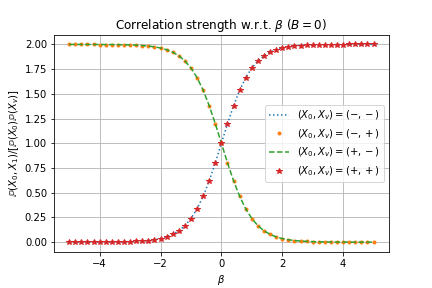
\includegraphics[width=9cm]{img/ising_x0_xv.png}
    \caption{
        We see the correlations for different $\beta$ values and $B=0$.
        If and only if $\frac{\pi_{\mu}(x_0, x_v)}{P(x_0)P(x_v)}=1$,
        i.e. $\pi_{\mu}(x_0, x_v) = P(x_0)P(x_v)$ for all $x_0$ and all $x_v$,
        does it mean that $X_0$ and $X_v$ are independent. This only happens at $\beta=0$. The further the values deviate from $1$,
        the more dependence there is. Additionally, We see that as $\beta$ gets
        larger, the $(+, +)$ and $(-, -)$ states are more preferred, and the opposite is true when $\beta$ gets more negative.}
    \label{Fig. x0-xv-correlation}
\end{figure}

$X_0$ and $X_v$ are identically distributed by admissibility. For $B=0$, both $X_0$ and $X_v$ are Bernoulli(1/2). It changes when $B\neq 0$. More
specifically, when $B\rightarrow\infty$, $X_0$ approaches deterministically spin-up. When $B\rightarrow\infty$, $X_0$ approaches deterministically spin-down.

\newpage

\begin{figure}[h]
    \centering
    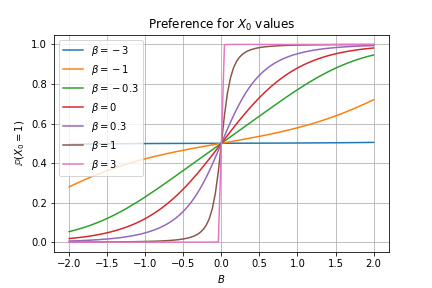
\includegraphics[width=9cm]{img/ising_x0_B.png}
    \caption{$X_0$ prefers $1$ when $B > 0$ and prefers $-1$ when $B < 0$. It is Bernoulli(1/2) when $B=0$}
    \label{Fig.ising-x0-B}
\end{figure}

\subsubsection{Investigating $\mathbb{P}_{\mu^*}(X_1, X_2)$}

\end{document}